\section{Realization}
\label{realisation}

Our implementation of our plug-in corresponds to the schema presented in Figure \ref{flowchart}. We can divide our work into 2 stages; first we analyzed and modelled the Android Intents, and then developed this model into abstract and concrete syntax. The second stage of development is where we transform our existing abstract syntax data into structured JDT and AST methods which will be called to perform our code generation. All the steps will be described in more details in this section.  

\begin{figure}[t]
\label{flowchart}
  \centering
    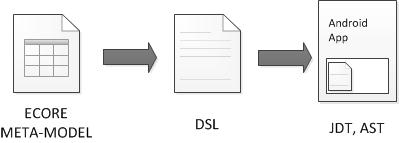
\includegraphics[width=0.65\textwidth]{flowchart}
  \caption{Flow Chart}
\end{figure}

We began by determining the DSL of Android Intents and developed our Ecore meta-model which reflected the DSL. Our DSL is based on several examples taken from Open Intents website\footnote{http://www.openintents.org/en/}, the default Android Intents included in Android, and finally the knowledge presented in the Section \ref{intents}. The final Ecore model is shown Figure \ref{meta-model}. Here "Model" is our root element that leads to an Intent. Each Intent has an action, category, and data which are described in Section \ref{intents}. It is specified by an Intent type: Standard, or Broadcast. If necessary it can contain multiple Extras, Permissions, and a single Callback.

\begin{figure}[t]
\label{meta-model}
  \centering
    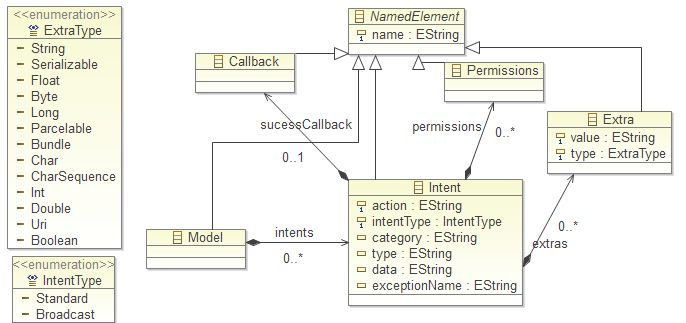
\includegraphics[width=0.9\textwidth]{metamodel}
  \caption{Meta-model of Intent}
\end{figure}

The second stage of development was to take this model and build the Xtext grammar. The final Xtext grammar we produced was based on the default grammar that was generated but with several modifications for simplification and the use of enumerated types. To test the grammar we developed several models based on some examples that we had previously chosen. This allowed us to make changes to both the Xtext grammar and the Ecore model when one or both did not suit the required data from the Intents. The developed models in our DSL are used as our database for the plug-in. An example of an Intent in our DSL is shown in the Listing \ref{dsl}.

{\footnotesize\begin{lstlisting}[escapechar=!,label=dsl,caption=Intent in DSL]
Intent "Action Send Text" {
	action "android.intent.action.SEND"
	category "android.intent.category.DEFAULT"
	type "text/plain"
	extras {
		String "android.intent.extra.TEXT" "Put your text here"
	}
},
\end{lstlisting}}

The plug-in uses Model-to-Model transformations, and for this purpose we use JDT and AST as explained in Section \ref{tools}. The database as defined in our abstract syntax is loaded, and the plug-in interface is built by iterating over the data. The interface allows a user to choose an Intent and generate the respective code in place where the cursor is in the editor window. This code is generated through a Model-to-Model transformation from the data held in the abstract syntax to the AST nodes.

This Model-to-Model transformation is largely obtained through using the generated model code that our Ecore model provides - it provides setters and getters for all properties of each class object, and also allows relationships defined in the Ecore model to be programatically called. Using a combination between the generated setup code provided with our Xtext DSL - IntentDslStandaloneSetup() - and the generated Java model code from our Ecore model, the plug-in quickly transforms our DSL model into actual Java object instances. The code shown in Listing \ref{loadingDsl} shows this loading and transformation.

{\footnotesize\begin{lstlisting}[label=loadingDsl,caption=Loading a DSL object into a standalone Java application]
public Model getModel() {
	Injector injector = new IntentDslStandaloneSetup().createInjectorAndDoEMFRegistration();
	XtextResourceSet resourceSet = injector.getInstance(XtextResourceSet.class);
	resourceSet.addLoadOption(XtextResource.OPTION_RESOLVE_ALL, Boolean.TRUE);
	Bundle bundle = Platform.getBundle("itu.dk.aamj.intentdsl.ui");
	URL fileURL = bundle.getEntry("gen/i.intentdsl");
	Resource resource = resourceSet.getResource(URI.createURI(fileURL.toString()), true);
	model = (Model) resource.getContents().get(0);
	return model;
}
\end{lstlisting}}

The plug-in is capable of handling the three different types of Intent identified; standard Activity Intents, broadcast Intents, and Intents with a callback. The plug-in provides several additional features to aid the developer: searching the database, exception handling, producing callback methods if required, and finally the AndroidManifest.xml file is modified with any required permissions. These additional features provide a quick and efficient experience for the developer, with intervention only required when the default settings produced should be modified. The final plug-in interface is shown in Figure \ref{codegeneratorview}.

\begin{figure}[t]
\label{codegeneratorview}
  \centering
    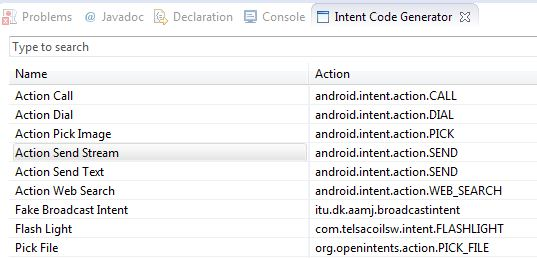
\includegraphics[width=\textwidth]{codegenerator}
  \caption{Final plug-in view}
\end{figure}

Listing \ref{generatedCode} shows an example of the generated code for an Intent which sends customized string to a non specified receiver. The AST of this generated code is shown in Figure \ref{intenttreeview}. To build the AST the Java code required is quite verbose, for example the code shown in Listing \ref{astjavacodesettype} adds the statement to set the type property of the intent - as shown on line two of Figure \ref{generatedCode}. Intents have several properties which can be set, and along with additional code required to build exception handling and callback receivers, the Java code required to build the necessary AST exceeds several hundred lines of code. This verboseness introduces increased complexity and maintainability issues into our plug-in, but could probably be reduced with further development and code encapsulation.

{\footnotesize\begin{lstlisting}[label=generatedCode,caption=Generated code of an Intent]
Intent ast = new Intent("android.intent.action.SEND");
ast.setType("text/plain");
ast.putExtra("android.intent.extra.TEXT", text);
startActivity(ast);		
\end{lstlisting}}

{\footnotesize\begin{lstlisting}[label=astjavacodesettype,caption=Java code to set type property]
// i.setType( value )
// intent = Java object of type Intent.
String intentType = intent.getType();
if(intentType != null) {

	StringLiteral data = ast.newStringLiteral();
	data.setLiteralValue(intentType);
	
	MethodInvocation methodInv = ast.newMethodInvocation();
	methodInv.setExpression(instanceName);
	methodInv.setName(ast.newSimpleName("setType"));
	methodInv.arguments().add(data);
	
	statementsList.add(ast.newExpressionStatement(methodInv));
	
}		
\end{lstlisting}}

\begin{figure}[t]
\label{intenttreeview}
  \centering
    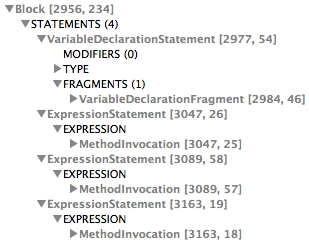
\includegraphics[width=.5\textwidth]{ast}
  \caption{AST of Generated Intent Code}
\end{figure}
